%% Section 3 — Conceptual Dimensions
\section{Conceptual Dimensions: Mapping Imaginaries and Strategic Visibility}
\label{sec:conceptual}

The conceptual dimension of a complex adaptive system, in the Phillips and Ritala (2019) sense, concerns how actors think about the system: the boundaries they draw, the perspectives they project, and the imaginaries through which the system becomes legible or illegible to itself and to outsiders. For data center assemblages, this dimension is where the ``cloud'' metaphor does its most consequential work. Operators actively construct an imaginary of placelessness — a representation of infrastructure as universal, weightless, and untethered from specific territories — and they do so through specific, analysable communicative acts. Two work packages address the conceptual dimension: WP1 through the textual register of corporate and territorial self-presentation, and WP2 through the visual register of satellite imagery and corporate photography.

\subsection{WP1: Corporate and Territorial Text}

Work Package 1 constructs a comparative textual corpus from two distinct registers of self-presentation: the corporate websites of major data center operators, and the Wikipedia articles for the cities and territories in which those operators are materially embedded. The two registers are treated as a diagnostic pair. Corporate websites are controlled communication — the imaginary the operator chooses to project. Wikipedia articles are community-assembled territorial description — a counter-register that reflects how a city, its residents, and its encyclopaedic record-keepers understand the infrastructure's presence in their place.

The collection infrastructure targets three page types per operator — sustainability pages, facility listing pages, and about pages — extracting plain text, structured metadata, image alt tags, and facility-geography links. A predefined keyword vocabulary spanning energy, water, carbon, location, sustainability, and community terms is applied at collection time, producing normalised frequency counts per page. The Wikipedia collection retrieves the full article for each city, parsing it into sections and flagging every sentence containing a reference to data center infrastructure, with particular attention to the Economy, Infrastructure, Environment, and Industry sections where such references are analytically significant.

The analytical logic rests on divergence: the gap between what the corporate register claims and what the territorial register records. An Environmental Claim Index (a weighted density score combining carbon, energy, sustainability, and water vocabulary) is computed for both sources per operator–city pairing, and the divergence between the two ECI scores is the primary output. A high corporate ECI paired with a low Wikipedia ECI operationalises what the notebook calls a greenwashing pattern — environmental claims decoupled from territorial accountability. A high energy-to-location ratio in corporate text signals an efficiency framing that abstracts spatial politics into technical performance. The disappearance of terms like ``planning,'' ``objection,'' ``noise,'' or ``neighbourhood'' from the corporate page is treated as analytically significant: their absence is the act of placelessness production.

The USA--Europe comparison sharpens the diagnostic. In Northern Virginia, operators describe the Loudoun County cluster in terms of network density, hyperscale capacity, and renewable energy commitments, constructing a territory of opportunity with minimal friction language. The Wikipedia record for Ashburn is beginning to accumulate territorial acknowledgement — data center references appearing in economic and infrastructure sections — but the encyclopaedic register still lags the pace of land-use contestation on the ground. In the Amsterdam case, the divergence scores function differently. The Dutch regulatory environment and the 2019--2022 moratorium episode have created a context in which operators cannot produce the cloud imaginary without acknowledging their territorial footprint. The sustainability vocabulary in Amsterdam-linked corporate materials is correspondingly denser — but the analytical question WP1 poses is whether that density reflects genuine territorial embeddedness or a more sophisticated absorption of territorial critique, one that speaks the language of green infrastructure while resisting the spatial specificity that community and planning actors demand.

A preliminary pipeline run against the three seed facilities (April 2026) produces ECI scores of 167.1 for AWS/Ashburn and 75.7 for Digital Realty/Dallas against Wikipedia ECI scores of 1.4 and 3.1 respectively, yielding divergence gaps of 165.7 and 72.6 (\Cref{fig:eci_divergence}). Equinix's corporate site returned no data, having blocked the scraper with a WAF --- itself a data point: strategic invisibility enacted at the technical layer. The magnitude of the AWS divergence is analytically striking: a corporate ECI more than 120 times the Wikipedia score is not consistent with genuine territorial embedding; it is consistent with imaginary production under low disclosure pressure.

\begin{fullwidth}
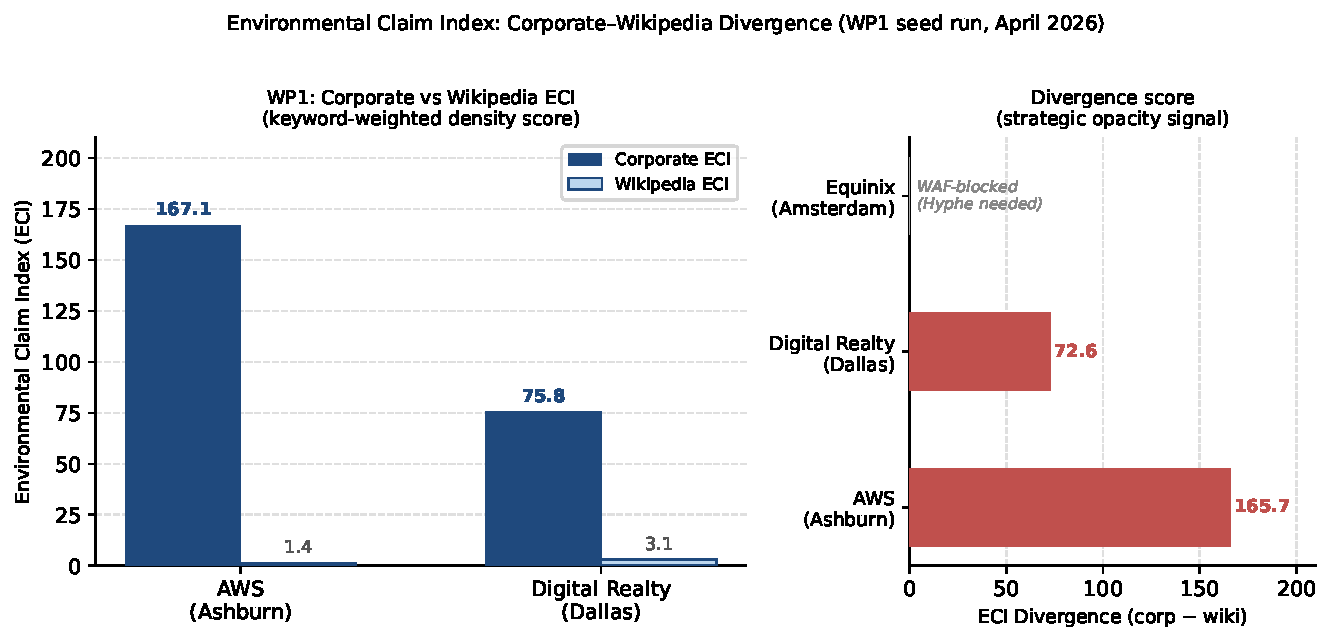
\includegraphics[width=\linewidth]{figures/wp1_eci_divergence}
\vspace{0.4em}
\captionof{figure}{WP1 seed results: Environmental Claim Index (ECI) for corporate websites versus Wikipedia articles (left), and ECI divergence gap per operator (right). A high divergence score indicates an operator constructing environmental claims that are decoupled from territorial accountability. Equinix's corporate site was blocked by a WAF, itself a finding. Data: pipeline run, April 2026.}
\label{fig:eci_divergence}
\end{fullwidth}

\subsection{WP2: Visual and Strategic Invisibility}

Data centers are designed, at considerable expense, to look like nothing. The suppression of windows, signage, and human scale is not an incidental feature of industrial economy but a deliberate act of visual engineering. WP2 treats this designed invisibility as a constitutive element of the assemblage rather than a communications strategy layered onto it: what operators choose not to show is as analytically significant as what they do show.

The work package operates across two parallel streams of visual material. The first is Sentinel-2 satellite imagery acquired at 10-metre resolution for a 500-metre bounding box around each facility coordinate — a state-derived, operator-independent account of the physical footprint that records building envelopes, cooling infrastructure, car parks, and spatial relationships to adjacent land uses that operators do not control and cannot redact. The second stream is corporate-published imagery scraped from operator websites: sustainability pages, facilities pages, and about-us sections, collected with full respect for robots.txt and assembled into per-operator manifests that record image files, alt text, and surrounding page context.

The analytical pipeline extracts Pillow-based visual metrics from each image — dimensions, aspect ratio, dominant colour — and assigns a content category: \textit{abstract} (server rooms, racks, logos, sustainability iconography), \textit{exterior} (building facades, campuses, cooling towers), or \textit{unknown}. Classification draws on alt text keyword matching as a baseline, with optional zero-shot CLIP or ResNet50 classification. From these labels a scalar \textit{visual abstraction score} — the ratio of abstract to total labelled images per operator — is computed. This score operationalises the degree to which an operator's visual self-presentation is decoupled from the material specificity of its facilities.

The abstraction score is not merely a measure of communications strategy. It is a governance claim. Visual substitution of abstract, placeless imagery for exterior location shots performs the cloud imaginary at the moment planning authorities and communities are contesting that framing. A jurisdiction comparison — operationalised through a Kruskal-Wallis test across facilities grouped by disclosure regime — tests whether visual abstraction is systematically associated with lighter regulatory environments. The predicted pattern, grounded in the comparative case: high abstraction in Loudoun County, where disclosure requirements are low and hyperscale anonymity is the default; lower abstraction in Amsterdam, where Dutch planning law and public debate have created a higher-disclosure environment in which operators face pressure to account for their footprint.

A first empirical pass of the satellite pipeline against the three seed facilities (April 2026) has yielded three analytical layers. Sentinel-2 RGB imagery at 10-metre resolution provides the baseline exterior record. Landsat 8/9 Land Surface Temperature (LST) composites for summer 2024 — derived from the ST\_B10 thermal band, converted to degrees Celsius at 30-metre resolution, across a 3\,km bounding box — make the thermal footprint of each facility visible as a heat signature: the consequence of round-the-clock cooling operations that operators do not publish and that no corporate image catalogue contains. VIIRS nighttime lights annual composites (NOAA DNB monthly V1, 2014--2024, 500-metre resolution, 10\,km radius) provide a longitudinal electricity-intensity record that is independent of operator disclosure.

The VIIRS time series produces a structurally revealing pattern. Ashburn shows a net increase in mean radiance of $+8.7\%$ between 2014 and 2024 --- the only jurisdiction in the seed sample with net positive growth (\Cref{fig:nightlights_ts}). Amsterdam records a $-9.2\%$ decrease over the same period, attributable to city-wide LED street lighting transition rather than reduced data center activity --- a measurement confound that is itself analytically instructive: in dense urban environments, the nighttime light proxy is attenuated by competing illumination sources and technology transitions, making the exurban Ashburn context the cleaner measurement environment. Dublin is flat at $-1.6\%$. The pattern is consistent with the WP3 land-use finding: deliberate spatial separation of the Ashburn cluster from residential settlement creates not only a governance gap but a cleaner physical signal.

The LST maps (\Cref{fig:lst_map}) make the thermal body of the assemblage visible at the site level. Cooling towers and server exhaust produce identifiable heat plumes extending beyond the facility perimeter — physical evidence of the energy flows that the cloud imaginary renders placeless. The contrast between the thermal profile of the Ashburn cluster --- an isolated heat source in an otherwise low-temperature exurban landscape --- and the Amsterdam facility --- whose thermal signature blends into the urban heat island, making it less legible as a discrete actor --- mirrors the governance contrast: physical embeddedness shapes the conditions under which communities can identify, attribute, and contest the infrastructure's impacts.

\begin{fullwidth}
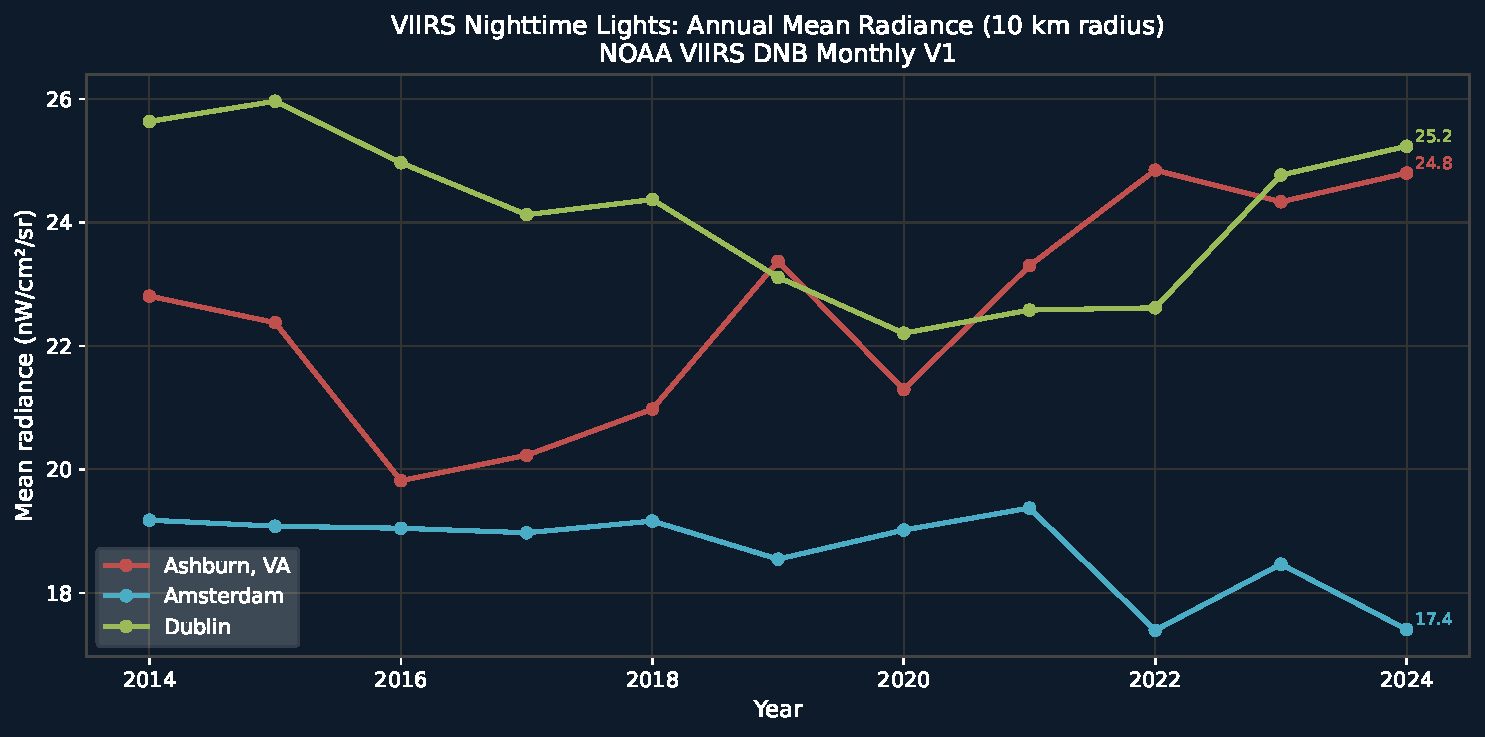
\includegraphics[width=\linewidth]{figures/wp2_nightlights_timeseries}
\vspace{0.4em}
\captionof{figure}{VIIRS nighttime lights: annual mean radiance (nW/cm\textsuperscript{2}/sr) within a 10\,km radius of each seed facility, 2014--2024 (NOAA VIIRS DNB Monthly V1, 500\,m resolution, Google Earth Engine). Ashburn is the only jurisdiction with net radiance growth ($+8.7\%$), consistent with data center cluster expansion in a low-background exurban context. Amsterdam's decrease ($-9.2\%$) reflects LED street lighting transition, a measurement confound that is more severe in dense urban environments. Data: GEE pipeline run, April 2026.}
\label{fig:nightlights_ts}
\end{fullwidth}

\begin{fullwidth}
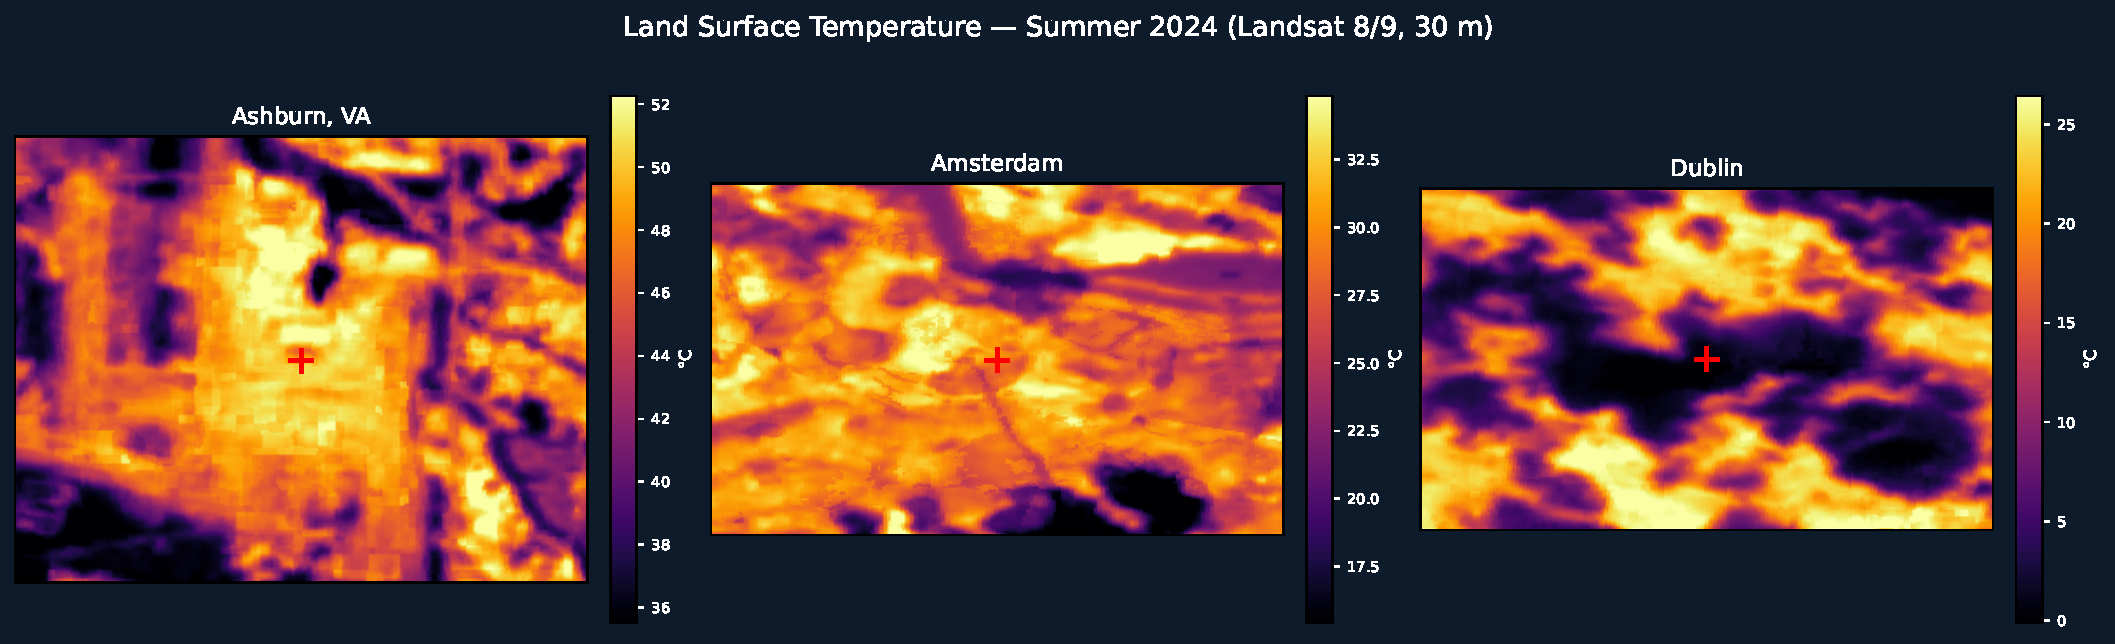
\includegraphics[width=\linewidth]{figures/wp2_lst_map}
\vspace{0.4em}
\captionof{figure}{Land Surface Temperature (LST) maps for the three seed facilities, summer 2024 composite (Landsat 8/9 Collection 2 Level-2, ST\_B10 band, June--August, $\leq 20\%$ cloud cover, 30\,m resolution, 3\,km bounding box). Red crosshairs mark facility centroids. The Ashburn facility sits within a discrete heat plume isolated from the surrounding low-temperature exurban landscape; Amsterdam and Dublin thermal signatures are embedded in the urban heat island. Data: GEE pipeline run, April 2026.}
\label{fig:lst_map}
\end{fullwidth}

The satellite record is, in this sense, the second measurement of the same gap that WP1 identifies in the textual record. Where WP1 finds a corporate ECI more than 120 times the Wikipedia score for Ashburn, WP2 finds a growing heat scar in the Virginia landscape that no corporate image catalogue contains. The operator narrates sustainability; the satellite records the thermal consequence of round-the-clock cooling. These are not independent findings that happen to be consistent: they are two modalities reaching the same sociotechnical fact --- the deliberate production of invisibility in one register does not alter the physical signature detectable in another. The divergence between what is claimed (clean, weightless, renewable infrastructure) and what is visible (an isolated, energy-intensive, thermally anomalous cluster) is the central analytical object of this work package, and it is only accessible through the juxtaposition of modalities that neither the textual nor the satellite record can achieve alone.

The four work packages and their mapping to CAS dimensions are summarised in \Cref{tab:wps}. Together, WP1 and WP2 map the conceptual dimension of the assemblage: the imaginaries through which data center infrastructure is made visible or invisible, the textual and visual acts through which territorial accountability is produced or evaded, and the variation in these across governance regimes that the CAS framing predicts will produce different structural and temporal outcomes.
